%% To submit your paper:
\documentclass[draft]{agujournal2019}
\usepackage{url} %this package should fix any errors with URLs in refs.
\usepackage{lineno}
\usepackage[inline]{trackchanges} %for better track changes. finalnew option will compile document with changes incorporated.
\usepackage{soul}
\linenumbers
%%%%%%%
% As of 2018 we recommend use of the TrackChanges package to mark revisions.
% The trackchanges package adds five new LaTeX commands:
%
%  \note[editor]{The note}
%  \annote[editor]{Text to annotate}{The note}
%  \add[editor]{Text to add}
%  \remove[editor]{Text to remove}
%  \change[editor]{Text to remove}{Text to add}
%
% complete documentation is here: http://trackchanges.sourceforge.net/
%%%%%%%

\draftfalse

\journalname{Geophysical Research Letters}


\begin{document}

%% ------------------------------------------------------------------------ %%
%  Title
%
% (A title should be specific, informative, and brief. Use
% abbreviations only if they are defined in the abstract. Titles that
% start with general keywords then specific terms are optimized in
% searches)
%
%% ------------------------------------------------------------------------ %%



\title{Duration of Individual Relativistic Electron Microbursts: A Probe Into Their Scattering Mechanism \textcolor{red}{... Better/shorter title?}}

%% ------------------------------------------------------------------------ %%
%
%  AUTHORS AND AFFILIATIONS
%
%% ------------------------------------------------------------------------ %%

% Authors are individuals who have significantly contributed to the
% research and preparation of the article. Group authors are allowed, if
% each author in the group is separately identified in an appendix.)

% List authors by first name or initial followed by last name and
% separated by commas. Use \affil{} to number affiliations, and
% \thanks{} for author notes.
% Additional author notes should be indicated with \thanks{} (for
% example, for current addresses).

% Example: \authors{A. B. Author\affil{1}\thanks{Current address, Antartica}, B. C. Author\affil{2,3}, and D. E.
% Author\affil{3,4}\thanks{Also funded by Monsanto.}}

\authors{M. Shumko\affil{1}, L.W. Blum\affil{2}, and A.B. Crew\affil{3}}


\affiliation{1}{NASA's Goddard Space Flight Center, Greenbelt, Maryland}
\affiliation{2}{University of Colorado Boulder, Boulder, Colorado}
\affiliation{3}{Johns Hopkins University Applied Physics Laboratory, Laurel, Maryland}

\correspondingauthor{M. Shumko}{msshumko@gmail.com}

%% Keypoints, final entry on title page.

%  List up to three key points (at least one is required)
%  Key Points summarize the main points and conclusions of the article
%  Each must be 100 characters or less with no special characters or punctuation and must be complete sentences

\begin{keypoints}
\item We identified relativistic microbursts observed by the SAMPEX satellite and quantified their duration
\item The microburst duration is shortest at midnight and longest at noon magnetic local times.
\item Whistler-mode chorus rising tone element duration has  a similar trend
\end{keypoints}

%% ------------------------------------------------------------------------ %%
%
%  ABSTRACT and PLAIN LANGUAGE SUMMARY
%
% A good Abstract will begin with a short description of the problem
% being addressed, briefly describe the new data or analyses, then
% briefly states the main conclusion(s) and how they are supported and
% uncertainties.

% The Plain Language Summary should be written for a broad audience,
% including journalists and the science-interested public, that will not have 
% a background in your field.
%
% A Plain Language Summary is required in GRL, JGR: Planets, JGR: Biogeosciences,
% JGR: Oceans, G-Cubed, Reviews of Geophysics, and JAMES.
% see http://sharingscience.agu.org/creating-plain-language-summary/)
%
%% ------------------------------------------------------------------------ %%

%% \begin{abstract} starts the second page

\begin{abstract}
In this study we used the Solar Anomalous and Magnetospheric Particle Explorer to identify relativistic, $>1$ MeV, electron microbursts and we quantified their duration. We found the shortest microbursts, with a median duration around 80 milliseconds, near midnight magnetic local time. Microburst duration increases through dawn and to noon magnetic local time, where the median microburst duration roughly doubles to 160 milliseconds. The increasing microburst duration trend in magnetic local time is similar to the whistler mode chorus rising tone element duration, shedding light into the microburst scattering mechanism.
\end{abstract}

\section*{Plain Language Summary}
\noindent Microbursts are a naturally occurring form of electron precipitation from the near-Earth space into the atmosphere. They are characterized by their short duration, typically defined to be less than a second, or sometimes as 100 milliseconds... Microburst impact on the atmosphere includes the degradation of Mesospheric Ozone through the production of Odd Nitrogen and Odd Hydrogen molecules... We don't know the details on how microburst electrons are scattered, but there is evidence that they are scattered by whistler-mode chorus rising tone elements... Talk about duration and how it is a probe into the scattering physics.

\section{Introduction}\label{intro}
Earth's outer radiation belt particle population is in constant flux, governed by many processes that affect particles via, for example: radial transport with injections from the magnetotail and ultra low frequency waves, local heating and loss into Earth's atmosphere due to wave-particle interactions \textcolor{red}{Cite Ripoll et al., 2019 "Particle Dynamics in the Earth's Radiation Belts: Review of Current Research and Open Questions"}. Whistler mode chorus (WMC) is just one type of plasma wave characterized by short ($\approx 100$ ms) rising tone elements, and perform a dual role in electron dynamics: accelerating electrons from $\approx 10$ keV injection energies up to MeV energies, and pitch angle scattering electrons into the atmosphere \cite<e.g.>{Li2009b, Thorne2010, Horne2003a, Summers2005}. One form of electron precipitation is microbursts: a transient and intense increase of electrons, with a $\approx 100$ ms duration, first observed by balloons in Earth's upper atmosphere, and later by satellites in low Earth orbit (LEO), and recently at high altitude near the magnetic equator \cite<e.g.>{Anderson1964, Blake1996, Lorentzen2001a, O'Brien2003,Douma2017, Kurita2016, Shumko2018b}.

\textcolor{blue}{Rewrite sentence. $\rightarrow$} The observed microburst electron energies span multiple orders of magnitude from tens of keV observed by, for example, \citeA{Datta1997} to $>1$ MeV observed by, for example, the Solar Anomalous Magnetospheric Particle Explorer (SAMPEX) by \citeA{Blum2015}. Spatially, microbursts are predominately observed outside the plasmapause; on the radiation belt footprints, $L\approx4-8$; and in the morning Magnetic Local Time (MLT) (0-12 hours MLT) \cite{Lorentzen2001a, Blum2015, O'Brien2003, Douma2017}. \textcolor{red}{If I keep the AE plot, I should discuss the microburst occurrence as a function of AE and Dst (Emma's and Paul's work).}

\textcolor{red}{Talk about their impact on the environment}

Electron microbursts and chorus waves were associated early on, due to their similar duration and similar occurrence distributions in MLT \cite<e.g.>{Lorentzen2001a}. Recently, \citeA{Breneman2017} directly linked a chorus rising tone element to a microburst observed by the Focused Investigation of Relativistic Electron Bursts: Intensity, Range, and Dynamics
(FIREBIRD-II) CubeSats \cite{Johnson2020} during a close magnetic conjunction. With this evidence, the particle precipitation community is largely in agreement that chorus waves scatter microbursts. A natural follow-on question is how. For example, it is still unclear if relativistic ($>1$ MeV) microbursts are scattered via cyclotron resonance at high magnetic latitudes, or a higher resonance harmonic near the magnetic equator \cite{Lorentzen2001a}. One way to address this question is by studying for how long microburst electrons are in resonance with a chorus wave. The resulting microburst duration, i.e. the microburst peak width in the time series data, is a probe into the conditions necessary to scatter microburst electrons. From our literature review, we found only qualitative estimates of the microburst duration. Therefore, we used the microbursts observed by the SAMPEX satellite to quantify the distribution of $>1$ MeV microburst duration. In this letter, we investigated the duration distribution as a function of: L-shell, MLT, and the Auroral Electrojet.

\section{Instrumentation}\label{instrumentation}
In this study we used the $>1$ MeV electron count data, taken by the Heavy Ion Large Telescope (HILT) instrument \cite{Klecker1993}, that was onboard the SAMPEX satellite \cite{Baker1993}. 

SAMPEX was launched in July 1992 and reentered Earth's atmosphere in November 2012. It was in a 520x670 km, $82^\circ$ inclination low Earth orbit. Broadly, the SAMPEX had two pointing modes: spin mode and orbit rate rotation (zenith pointing) modes. To avoid the compounding effects due to the variable pitch angles sampled in the spin mode, we only used the zenith pointing mode data.

We used the HILT electron data, sampled at a 20 ms cadence (state4 in the data archive), that was taken between 1997 and 2012. The HILT instrument consisted of a large rectangular chamber with the apperture on one end, and 16 solid state detectors on the other. The electron counts accumulated over 20 ms were summed from all of the solid state detectors and used in this study.

\section{Methodology}\label{methodology}

To estimate the microburst duration we first identified microbursts and then we fit them with a Gaussian model with a linear trend to quantify the duration for each microburst.

\subsection{Microburst Identification}\label{microburst_id}
We identified microbursts using the burst parameter defined by \citeA{O'Brien2003} and used in numerous other microburst studies with SAMPEX \cite<e.g.>{Douma2017}. Assuming Poisson probability for the observed electron counts, the burst parameter is the number of standard deviations of a foreground signal above the background, expressed as
\begin{equation}
n_\sigma = \frac{N-A}{\sqrt{A+1}}
\end{equation} where $N$ is the number of foreground electron counts (microburst or otherwise), and $A$ is the centered running average background counts. The $1$ in the denominator prevents a division by 0 error. In \citeA{O'Brien2003}, and in the results in this study, $N$ was summed over 0.1 seconds and is called $N_{100}$, while $A$ was summed over 0.5 seconds and is called $A_{500}$.  Henceforth we will specify the time window with the subscript for $N$ and $A$. Times when $n_\sigma > 10$ are classified as microburst times, and the peak count rate in each time interval is saved as a microburst to our data set. With $A_{500}$ and $N_{100}$, we detected a total of 256,764 microbursts over the 15 year period from 1997 to 2012. Four examples of microbursts are shown in Fig. \ref{fig1} by the solid black curves.

\textcolor{blue}{Check the argument for clarity} The choice of $A$ determines the sensitivity of the burst parameter to microbursts of various durations (widths). This sensitivity is best illustrated with an example. Given a 1-second wide microburst, if we use $A_{500}$, the centered average background at the microburst time is skewed towards the microburst peak and the microburst's $\mathrm{bp}$ is reduced, potentially below the detection threshold. On the other hand, if we use $A_{1000}$, the centered running background will be relatively less elevated at the microburst time so it has a greater $\mathrm{bp}$ and is more likely to be detected. In other words, $bp$ will be relatively larger for $A_{1000}$ than $A_{500}$. This sensitivity manifests itself as a bias towards detecting narrower microbursts that we will address later in this study. 

\begin{figure}
\noindent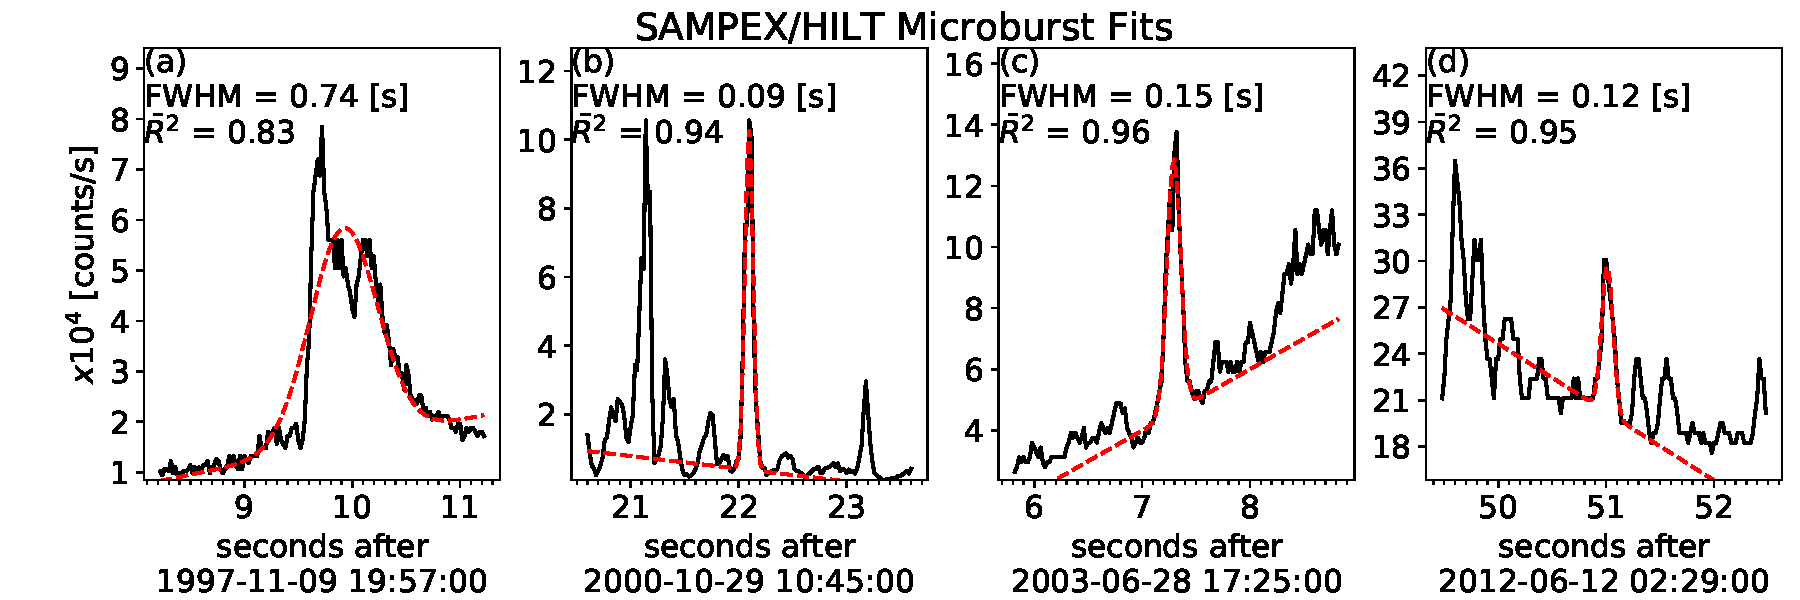
\includegraphics[width=\textwidth]{figures/fig1.pdf}
\caption{Example $>1$ MeV microbursts shown by the black lines, and the fits shown by the dashed red lines. The fit full width at half maximum (FWHM) and the $\bar{R}^2$ goodness of fit metric is annotated in each panel. Microbursts with $\bar{R}^2 > 0.9$ were used for this study. The major time ticks are at every second, while the minor ticks are at every 100 milliseconds.}
\label{fig1}
\end{figure}

\subsection{Microburst Duration}
We estimated the microburst duration using two methods that yielded similar results: the duration at half of the microburst's topographic prominence and duration from a Gaussian fit.

The topographic prominence is a simple and robust method to estimate the microburst duration used to identify curtains a similar-looking type of precipitation \cite{Shumko2020b}. It is defined as the duration at half of the microburst topographic prominence: the height of the microburst relative to the maximum of the two minima on either side of the microburst peak. On each side of the microburst peak, the minima are searched for between the microburst and a higher peak on that side. While the topographic prominence method of estimating microburst durations is simple and robust, one of its downsides is its inability to automatically verify that the duration is representative of a single microburst. Therefore, we also fit microbursts with a Gaussian, and used the $R^2$ goodness of fit metric to filter out bad duration estimates.

The other method that we use to estimate the microburst duration is fitting a Gaussian shape to microbursts. The advantage of this method is that it allows us to evaluate the fit using a goodness of fit metric. By screening out bad fits, we exclude superposition of multiple microbursts that will unintentionally bias our microburst duration estimate.

We assumed a Gaussian superposed with a linear trend fit model. The Gaussian models the shape of the microburst; while the linear trend accounts for the electrons that are either trapped or quasi-trapped in the drift loss cone. The fit model is defined as:
\begin{equation}
c(t | A, t_0, \sigma, c_0, c_1) = A e^{-\frac{(t-t_0)^2}{2\sigma^2}} + c_0 + c_1 t
\end{equation} \textcolor{red}{Reconsider variable names...} where $A$, $t_0$, and $\sigma$ are the Gaussian amplitude, center time, and standard deviation; while the $c_0$ and $c_1$ are the background count intercept and slope. The fit was applied over a number of data points determined by the maximum of either: 4x topographic prominence width or 0.5 seconds. A challenge to any robust and automated nonlinear regression algorithm is guessing the initial parameters. The initial parameter guesses for the Gaussian are provided by the topographic prominence and topographic duration estimates. The two linear trend initial parameters were: $c_0=\mathrm{median(counts)}$ and $c_1=0$. The optimal fit parameters were found using scipy's \url{curve_fit()} function in Python. We defined the microburst duration as the full width at half maximum (FWHM) of the microburst peak, defined as
\begin{equation}
\mathrm{FWHM} = 2\sqrt{2 \ln{2}} \sigma.
\end{equation}

To evaluate the fit, we used the $R^2$ goodness of fit metric. $R^2$ is defined as
\begin{equation}
R^2 = 1 - \frac{SS_{res}}{SS_{mean}} = 1 - \frac{\sum{(c_i-f_i)^2}}{\sum{(c_i-\bar{c})^2}}
\end{equation} where $SS_{res}$ is the sum of the squared residuals between the observed counts $c_i$ and the fit counts $f_i$ for each time stamp, and $SS_{mean}$ is the sum of the squared residuals between $c_i$ and the mean of the counts, $\bar{c}$.

One interpretation of $R^2$ is: fractionally how much better the variance in the data is explained by the model fit, compared to the null hypothesis horizontal line at $\bar{c}$. $R^2$ values vary from $1$ when the fit perfectly describes the variance in the data, to $-\infty$ for poor fits (a fit can be much worse than the mean null hypothesis).

To account for overfitting that results from the variable number of data points used for each fit, the adjusted $R^2$, $\bar{R}^2$, was used. It is defined as

\begin{equation}
\bar{R}^2 = 1 - (1-R^2) \frac{n-1}{n-p-1}
\end{equation} where $n$ is the number of data points fit, and $p$ is the number of parameters. Intuitively, $n-1$ is the number of degrees of freedom for the null hypothesis, and $n-p-1$ is the degrees of freedom for the fit model. Fits with $\bar{R}^2 > 0.9$ are considered good fits and are used for the rest of this analysis. We compared the microburst duration estimated with the prominence and fit methods. With the $\bar{R}^2 > 0.9$ constraint, we found that for $85\%$ of microbursts, the duration estimated by both methods agreed to within $25\%$.

Figure \ref{fig1}a shows an example of two superposed microbursts that had a fit $\bar{R}^2 = 0.83$ that were excluded from this study. On other hand, Fig. \ref{fig1}b-d show microbursts that were included in this study because the fit $\bar{R}^2 > 0.9$.

Lastly, Fig. \ref{fig1}c,d demonstrate the necessity of the linear fit to account for the changing background. The linear fit accounts for the non-zero mean background counts and the different amplitudes of the edges of the Gaussian. Of the 256,764 detected microbursts, 109,231 had $R^2 > 0.9$ and are used for the remainder of this study.

\section{Results}\label{results}
The well-fit microbursts are used to quantify the distribution of microburst duration (FWHM) for all microbursts, as a function of L and MLT, and as a function of the Auroral Electroject (AE). We begin with the overall microburst distribution.

Figure \ref{figX} shows the distribution of all well-fit microbursts. This distribution is peaked with the median at 98 ms and quickly drops off. The interquartile range spans about a factor of two in microburst duration, from 67 to 140 ms. 

\begin{figure}
\noindent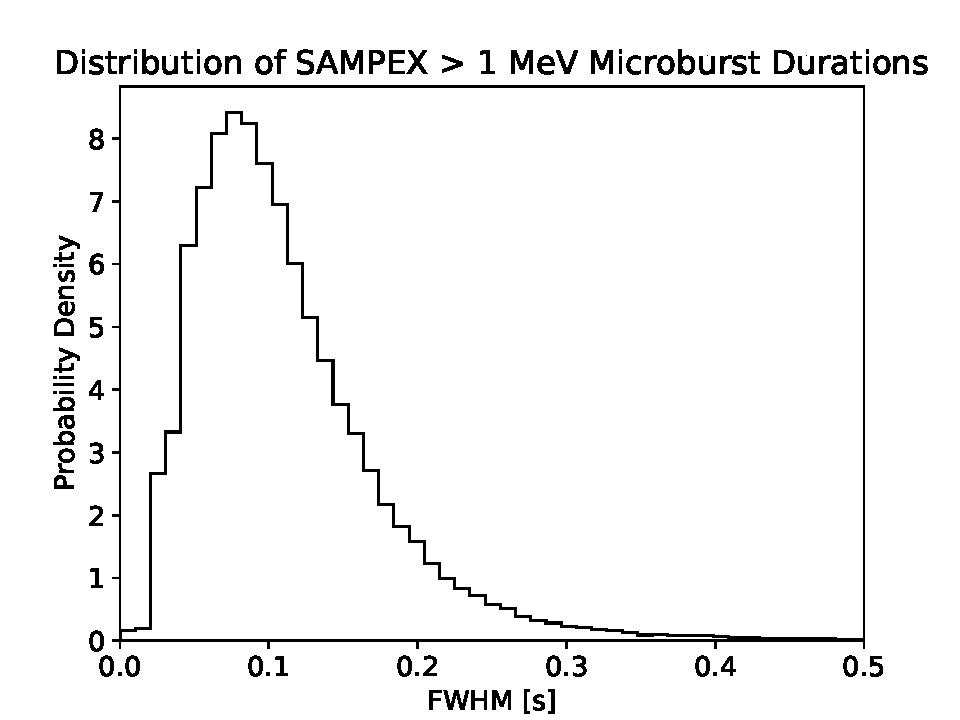
\includegraphics[width=\textwidth]{figures/figX.pdf}
\caption{The distribution of all microburst full width at full maximum (FWHM). \textcolor{red}{Maybe merge this plot with the AE plot?}}
\label{figX}
\end{figure}

Figure \ref{fig2} shows the joint distribution of microburst duration as a function of L and MLT. Figure \ref{fig2}a-c show the 25\%, 50\%, and 75\% percentiles of microbursts in each L-MLT bin. The sparse bins with less than 100 well-fit microbursts are white. For reference, Fig. \ref{fig2}d shows the number of well-fit microbursts observed as a function of L and MLT.

In Fig. \ref{fig2}, the microburst duration trend is almost identical for the different percentiles, but lets focus on the median distribution, Fig. \ref{fig2}b. In MLT, the median microburst duration increases by a factor of two: from 80 ms at midnight to 160 ms at noon. In L-shell, the median microburst duration slightly increases with L shell, most apparent near midnight MLT. To disentangle the L and MLT distribution, Fig. \ref{fig3} shows the marginalized distributions; MLT was marginalized out in Fig. \ref{fig3}a and L-shell was marginalized out in Fig. \ref{fig3}b. Figure \ref{fig3}a shows a slight broadening of the microburst duration at higher L-shells; in contrast to Fig. \ref{fig3}b that clearly shows that the microburst duration increases from midnight to noon MLT.

Lastly, we investigated the dependence of microburst duration as a function of geomagnetic activity. To be consistent with the prior wave and microburst studies, we use the Auroral Electrojet (AE) index to quantify the level of geomagnetic disturbance. We adopt the same three AE intensity levels used in prior studies, such as \citeA{Li2009a}, \citeA{Douma2017}, and \citeA{Meredith2020}: $\mathrm{AE} < 100$, $100 < \mathrm{AE} < 300$, and $300 < \mathrm{AE} < 1000$, in nanotesla units. Figure \ref{fig4} shows the distribution of microburst duration as a function of AE. This distribution is similar across the three AE intensity levels. However, the distribution is more prominently peaked at 0.1 s at the highest intensity level.

\begin{figure}
\noindent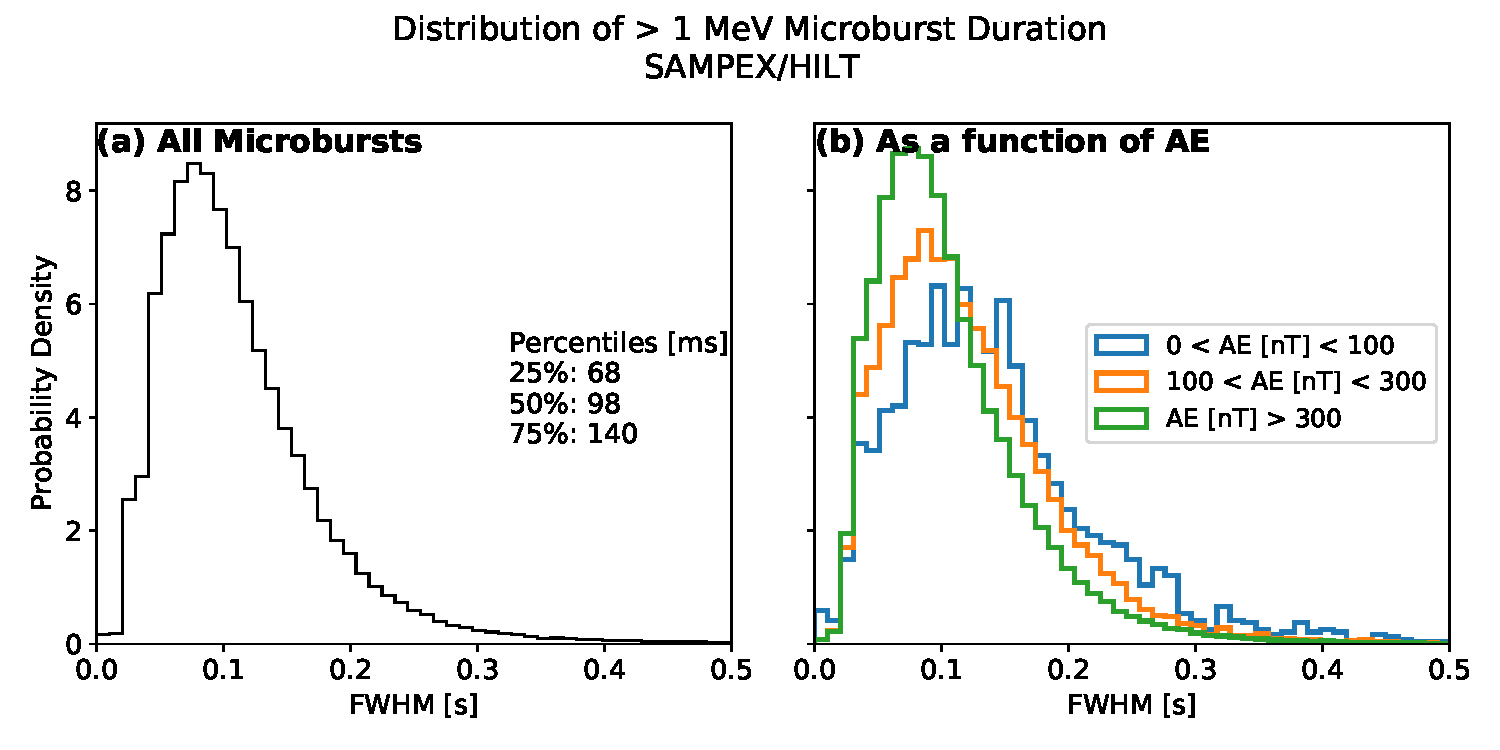
\includegraphics[width=\textwidth]{figures/fig2.pdf}
\caption{The joint distributions of microburst duration (FWHM) as a function of L and MLT. In each L-MLT bin with more than 100 good microburst fits, the 25th, 50th, and 75th percentiles of the duration were calculated and shown in panels a-c, respectively. The white bins in panels a-c have less than 100 good microburst fits. Panel d shows the distribution of the number of microbursts with 0 microbursts shown with the white bins.}
\label{fig2}
\end{figure}

\begin{figure}
\noindent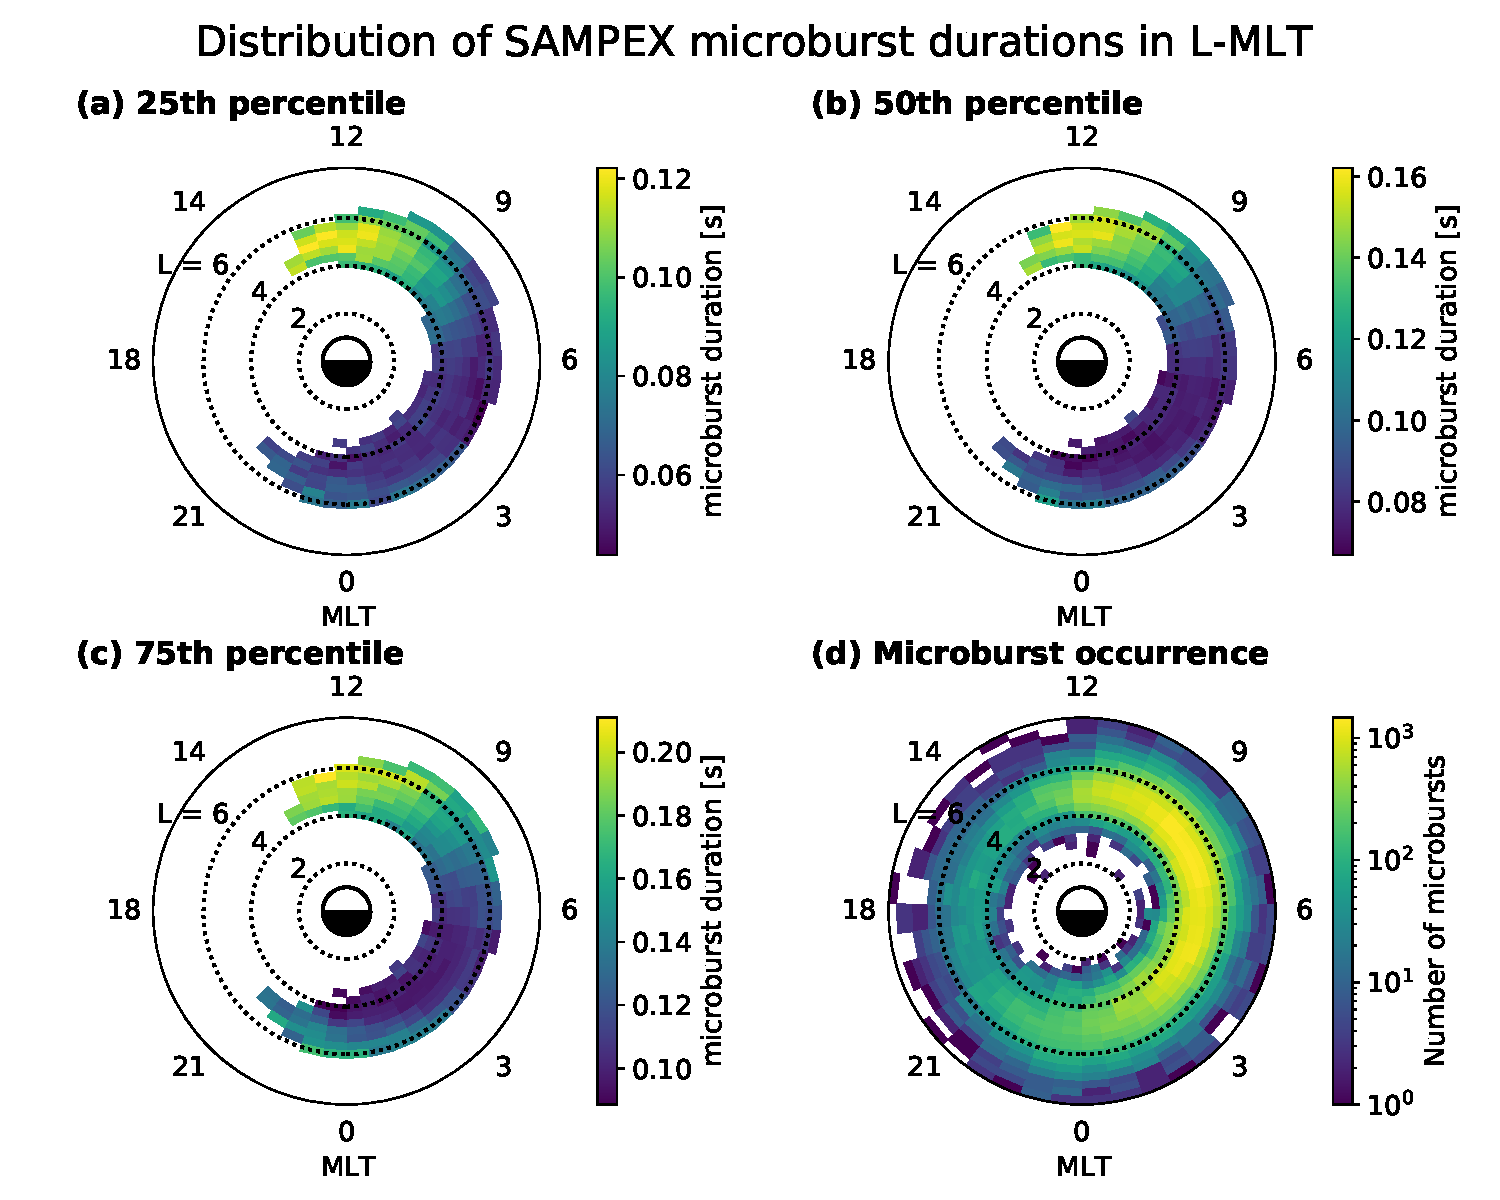
\includegraphics[width=\textwidth]{figures/fig3.pdf}
\caption{The marginalized distributions of the number of microbursts as a function of microburst duration (FWHM) and L shell in panel a and MLT in panel b.}
\label{fig3}
\end{figure}

\begin{figure}
\noindent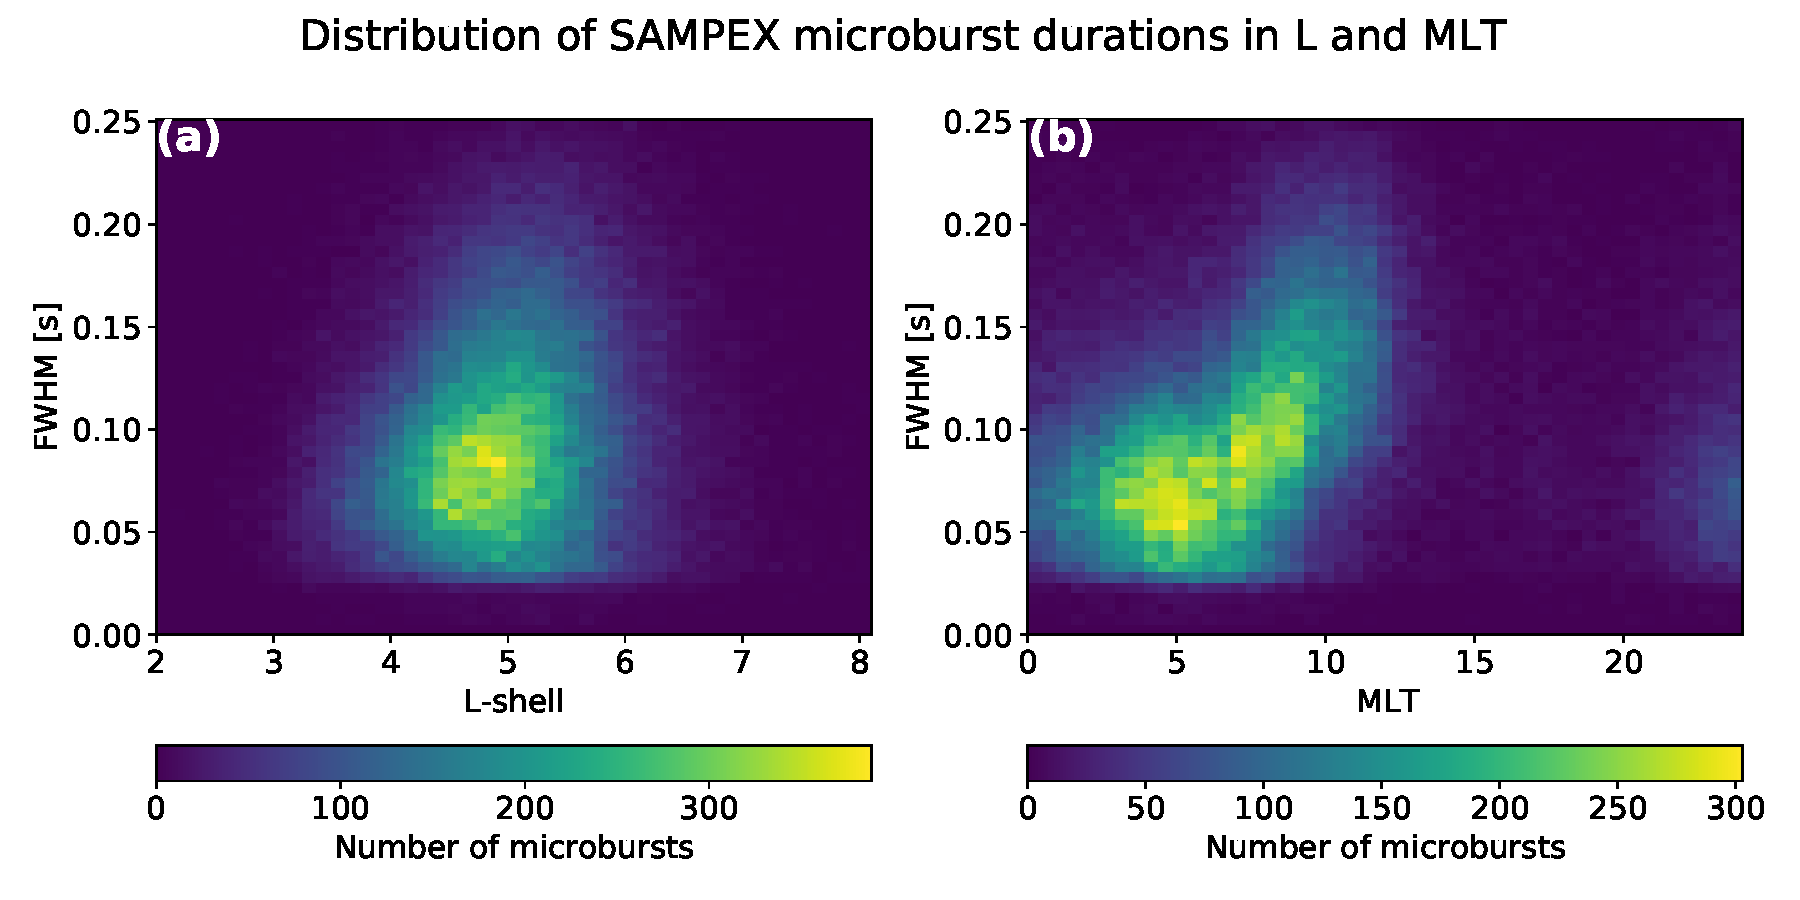
\includegraphics[width=\textwidth]{figures/fig4.pdf}
\caption{The distribution of the microburst duration (FWHM) for three ranges of the Auroral Electroject: $\mathrm{AE} < 100$, $100 < \mathrm{AE} < 300$, and $300 < \mathrm{AE} < 100$ nT in Panels a-c, respectively. The x- and y-axis share identical limits between the three panels.}
\label{fig4}
\end{figure}

\section{Discussion and Conclusions}\label{discussion}
\textcolor{blue}{
\textbf{Outline}
\begin{enumerate}
    \item Compare to prior microburst width estimates.
    \item Comment that microbursts at lower energy are wider (data + model). The cited microburst widths are dependent by the energy channel of the instrument. 
    \item Compare to chorus rising tone element duration trends.
    \item A few concluding remarks.
\end{enumerate}
}

To address the burst parameter preferential bias to narrower microbursts, as introduced in section \ref{microburst_id}, we ran the microburst identification algorithm on the data using three background values: $A_{500}$, $A_{1000}$, and $A_{1000}$. As described in section \ref{microburst_id}, an detection algorithm who's centered running average is over wider time periods will be more sensitive to wider and less prominent microbursts. Therefore we can identify the bias if there is a relative excess of longer duration microbursts when the average time was increased. We found no such excess for microburst data sets that were made using $A_{1000}$, and $A_{1000}$. Therefore, we believe that $>1$ MeV microbursts are truly narrower than 250 ms and the $A_{500}$ is adequate to identify $>1$ MeV microbursts.

The microburst duration distribution, shown in Fig. \ref{fig2} shows that the median microbust duration is approximately 100 ms, in agreement with prior studies \textcolor{red}{Cite}. Hoever, we found an unexplored trend in the literature where the microburst duration at lower energies is wider \cite<e.g.>{Johnson2020, Shumko2020a}. This trend is consistent with recent modeling by \citeA{Chen2020} and \citeA{Miyoshi2020}, but needs to be fully explored with energy-resolved measurements provided by, for example, FIREBIRD-II.

\textcolor{blue}{First talk about that the distribution is fairly narrow around one seconds (mention longer for low energy, also predicted in papers) and that there's no difference in L but there is a difference in MLT and now let's look into how the distribution of microverts and course waves compare in the local time Now the rising tone element duration has very similar trend as a doubles roughly from midnight to noon magnetic local time However in the work done by longing chen they show that the micro reservation should be governed by some sort of a diffusion curves stuff but that depends or controlled directly by the bandwidth of the wave.}

\textcolor{red}{Discuss rising tone preprties from Sheng and Teng papers, relate to the Miyoshi and Chen microburst pepers.}

%%%%%%%%%%%%%%%%%%%%%%%%%%%%%%%%
%% Optional Appendix goes here
%
% The \appendix command resets counters and redefines section heads
%
% After typing \appendix
%
%\section{Here Is Appendix Title}
% will show
% A: Here Is Appendix Title
%
%\appendix
%\section{Here is a sample appendix}

\acknowledgments
We are thankful for the engineers and scientists who made the SAMPEX mission possible. M. Shumko is thankful for the support provided by the NASA Postdoctoral Program at the NASA’s Goddard Space Flight Center, administered by Universities Space Research Association under contract with NASA. \textcolor{red}{Lauren's and Alex's funding sources} The SAMPEX HILT and attitude data are located at \url{http://www.srl.caltech.edu/sampex/DataCenter/data.html} and the minute cadence Auroral Electroject data is located at \url{ftp://ftp.ngdc.noaa.gov/STP/GEOMAGNETIC_DATA/INDICES/AURORAL_ELECTROJET/ONE_MINUTE/}.
The analysis software is archived at \textcolor{red}{\url{https://github.com/mshumko/sampex_microburst_widths}}.


%% ------------------------------------------------------------------------ %%
%% References and Citations

%%%%%%%%%%%%%%%%%%%%%%%%%%%%%%%%%%%%%%%%%%%%%%%
%
% \bibliography{<name of your .bib file>} don't specify the file extension
%
% don't specify bibliographystyle
%%%%%%%%%%%%%%%%%%%%%%%%%%%%%%%%%%%%%%%%%%%%%%%

\bibliography{refs.bib}



%Reference citation instructions and examples:
%
% Please use ONLY \cite and \citeA for reference citations.
% \cite for parenthetical references
% ...as shown in recent studies (Simpson et al., 2019)
% \citeA for in-text citations
% ...Simpson et al. (2019) have shown...
%
%
%...as shown by \citeA{jskilby}.
%...as shown by \citeA{lewin76}, \citeA{carson86}, \citeA{bartoldy02}, and \citeA{rinaldi03}.
%...has been shown \cite{jskilbye}.
%...has been shown \cite{lewin76,carson86,bartoldy02,rinaldi03}.
%... \cite <i.e.>[]{lewin76,carson86,bartoldy02,rinaldi03}.
%...has been shown by \cite <e.g.,>[and others]{lewin76}.
%
% apacite uses < > for prenotes and [ ] for postnotes
% DO NOT use other cite commands (e.g., \citet, \citep, \citeyear, \nocite, \citealp, etc.).
%



\end{document}



More Information and Advice:

%% ------------------------------------------------------------------------ %%
%
%  SECTION HEADS
%
%% ------------------------------------------------------------------------ %%

% Capitalize the first letter of each word (except for
% prepositions, conjunctions, and articles that are
% three or fewer letters).

% AGU follows standard outline style; therefore, there cannot be a section 1 without
% a section 2, or a section 2.3.1 without a section 2.3.2.
% Please make sure your section numbers are balanced.
% ---------------
% Level 1 head
%
% Use the \section{} command to identify level 1 heads;
% type the appropriate head wording between the curly
% brackets, as shown below.
%
%An example:
%\section{Level 1 Head: Introduction}
%
% ---------------
% Level 2 head
%
% Use the \subsection{} command to identify level 2 heads.
%An example:
%\subsection{Level 2 Head}
%
% ---------------
% Level 3 head
%
% Use the \subsubsection{} command to identify level 3 heads
%An example:
%\subsubsection{Level 3 Head}
%
%---------------
% Level 4 head
%
% Use the \subsubsubsection{} command to identify level 3 heads
% An example:
%\subsubsubsection{Level 4 Head} An example.
%
%% ------------------------------------------------------------------------ %%
%
%  IN-TEXT LISTS
%
%% ------------------------------------------------------------------------ %%
%
% Do not use bulleted lists; enumerated lists are okay.
% \begin{enumerate}
% \item
% \item
% \item
% \end{enumerate}
%
%% ------------------------------------------------------------------------ %%
%
%  EQUATIONS
%
%% ------------------------------------------------------------------------ %%

% Single-line equations are centered.
% Equation arrays will appear left-aligned.

Math coded inside display math mode \[ ...\]
 will not be numbered, e.g.,:
 \[ x^2=y^2 + z^2\]

 Math coded inside \begin{equation} and \end{equation} will
 be automatically numbered, e.g.,:
 \begin{equation}
 x^2=y^2 + z^2
 \end{equation}


% To create multiline equations, use the
% \begin{eqnarray} and \end{eqnarray} environment
% as demonstrated below.
\begin{eqnarray}
  x_{1} & = & (x - x_{0}) \cos \Theta \nonumber \\
        && + (y - y_{0}) \sin \Theta  \nonumber \\
  y_{1} & = & -(x - x_{0}) \sin \Theta \nonumber \\
        && + (y - y_{0}) \cos \Theta.
\end{eqnarray}

%If you don't want an equation number, use the star form:
%\begin{eqnarray*}...\end{eqnarray*}

% Break each line at a sign of operation
% (+, -, etc.) if possible, with the sign of operation
% on the new line.

% Indent second and subsequent lines to align with
% the first character following the equal sign on the
% first line.

% Use an \hspace{} command to insert horizontal space
% into your equation if necessary. Place an appropriate
% unit of measure between the curly braces, e.g.
% \hspace{1in}; you may have to experiment to achieve
% the correct amount of space.


%% ------------------------------------------------------------------------ %%
%
%  EQUATION NUMBERING: COUNTER
%
%% ------------------------------------------------------------------------ %%

% You may change equation numbering by resetting
% the equation counter or by explicitly numbering
% an equation.

% To explicitly number an equation, type \eqnum{}
% (with the desired number between the brackets)
% after the \begin{equation} or \begin{eqnarray}
% command.  The \eqnum{} command will affect only
% the equation it appears with; LaTeX will number
% any equations appearing later in the manuscript
% according to the equation counter.
%

% If you have a multiline equation that needs only
% one equation number, use a \nonumber command in
% front of the double backslashes (\\) as shown in
% the multiline equation above.

% If you are using line numbers, remember to surround
% equations with \begin{linenomath*}...\end{linenomath*}

%  To add line numbers to lines in equations:
%  \begin{linenomath*}
%  \begin{equation}
%  \end{equation}
%  \end{linenomath*}



